% Rozdział 6 – konstrukcje i ekstrema


\theory{Konstrukcje}

\noindent
W tym rozdziale będziemy obracać się wokół zadań, które polegają na konstruowaniu pewnych obiektów, spełniających pewne warunki. Najpierw przyjrzymy się zadaniu, w którym mamy wyznaczyć pewne maksimum. W takiej sytuacji musimy zarówno pokazać przykład, że maksimum jest osiągane, jak i udowodnić, że nie da się osiągnąć większej wartości.

\vspace{10px}

\heading{Przykład 1}

\noindent
Wyznaczyć maksymalną liczbę skoczków, które można umieścić na szachownicy $8\times8$, aby żadne dwa z nich się nie biły.

\heading{Rozwiązanie}

\noindent
Wykażemy, że szukaną liczbą jest $32$.\\
Najpierw pokażemy, że istotnie można postawić tyle skoczków na szachownicy. Zauważmy, że rozpatrując standardowe kolorowanie szachownicy i stawiając skoczki na każdym z 32 pól jednego koloru, żadne dwa z nich nie będą się biły.

\begin{center}
    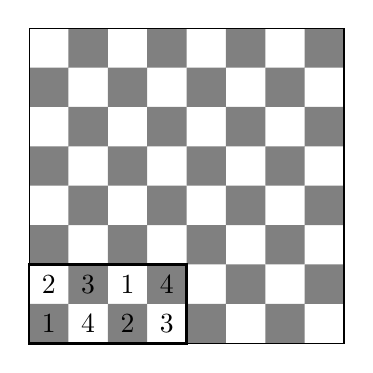
\begin{tikzpicture}[x=1cm, scale=0.5]
    \foreach \y in {0,2,...,6}{
        \foreach \x in {0,2,...,6}{
            \fill[black!50] (\x,\y) rectangle (1+\x,1+\y) rectangle (2+\x,2+\y);}}
    \node at (0.5,0.5) {1};
    \node at (2.5,1.5) {1};
    \node at (0.5,1.5) {2};
    \node at (2.5,0.5) {2};
    \node at (1.5,1.5) {3};
    \node at (3.5,0.5) {3};
    \node at (1.5,0.5) {4};
    \node at (3.5,1.5) {4};
    \draw (0,0)--(8,0)--(8,8)--(0,8)--cycle;
    \draw[line width=1] (0,0)--(4,0)--(4,2)--(0,2)--cycle;
    \end{tikzpicture}
\end{center}

\noindent
Podzielmy szachownice na $8$ prostokątów o wymiarach $4\times2$ -- takich jak na rysunku. Wykażemy, że wewnątrz każdego prostokąta mogą stanąć co najwyżej cztery skoczki. Istotnie – numerując pola tak jak na rysunku, nie jest możliwe aby na obu polach z tym samym numerem stały skoczki. Więc na całej szachownicy mogą stanąć co najwyżej $8 \cdot 4 = 32$ skoczki.

\qed

\vspace{5px}

\noindent
W powyższym zadaniu konieczne było zarówno udowodnienie, że nie da się postawić więcej niż $32$ skoczków, jak i wykazanie, że istnieje szukane ustawienie $32$ skoczków. W tego typu problemach warto uważnie poszukać maksymalnego ustawienia, gdyż w przypadku jego przeoczenia, nasze próby dowodzenia, że znaleziona konfiguracja jest maksymalna będą bezsensowne. 

\vspace{10px}

% to zadanie ma pokazać analizę małych przypadków
%Source: https://om.mimuw.edu.pl/static/app_main/camps/oboz2018.pdf zadanie 1
\heading{Przykład 2}

\noindent
Niech $S(k)$ oznacza sumę cyfr liczby $k$ w zapisie dziesiętnym. Dodatnią liczbę całkowitą~$n$ nazwiemy \textit{piękną} jeśli zachodzi równość $S(n) = S(n^2)$. Wyznaczyć wszystkie wartości jakie przyjmuje $S(n)$ dla liczb pięknych n.

\newpage

\heading{Rozwiązanie}

\noindent
W rozwiązaniu poniższego zadania potrzebna będzie obserwacja, że suma cyfr liczby $k$ daje taką samą resztę z dzielenia przez $9$ jak liczba $k$. Mamy
\[
    n^2 \equiv S(n^2) = S(n) \equiv n \pmod{9}.
\]

\noindent
Zauważam, że jest to możliwe jedynie dla $n \equiv 0, 1 \pmod{9}$ -- wystarczy sprawdzić wszystkie możliwe $n$. Stąd $S(n) \equiv 0, 1 \pmod{9}$.

\vspace{5px}

\noindent
Po otrzymaniu powyższej obserwacji można postawić hipotezę, że dla wszystkich liczb dodatnich postaci $k \equiv 0, 1 \pmod{9}$ istnieje liczba piękna $n$, że $S(n) = k$. Aby zweryfikować, czy hipoteza ma sens warto sprawdzić, czy jest ona prawdziwa dla kilku małych wartości~$k$. Łatwo sprawdzić, że liczby $9$ i $10$ są piękne oraz $S(9) = 9$ i $S(10) = 1$. Poszukując większych wartości $S(n)$ dla liczb pięknych otrzymujemy $S(99) = 18$ i ${S(199) = 19}$. Łatwo też sprawdzić, że $99$ i $199$ są piękne. Te obserwacje, poczynione na kilku najmniejszych wartościach, naprowadzają nas na dalszą część rozwiązania.

\vspace{5px}

\noindent
Rozpatrzmy liczbę $a = 10^{k + 1} - 1$. Wówczas
\[
    S(a) = S(\underbrace{99...9}_{k+1}) = 9(k + 1) = S(\underbrace{99...9}_{k}8\underbrace{00...0}_{k}1) = S(10^{2k + 2} - 2\cdot 10^{k + 1} + 1) = S(a^2).
\]
Następnie weźmy liczbę $b = 2 \cdot 10^{k} - 1$. Wówczas
\[
    S(b) = S(1\underbrace{99...9}_{k}) = 9k + 1 = S(3\underbrace{99...9}_{k-1}6\underbrace{00...0}_{k-1}1) = S(4\cdot 10^{2k} - 4\cdot 10^{k} + 1) = S(b^2).
\]
Zauważamy, że dla dowolnej dodatniej liczby całkowitej $k$ liczby $a$, $b$ są piękne oraz ${S(a) = 9(k + 1)}$ i $S(b) = 9k + 1$.

\noindent
Łącząc powyższe wnioski otrzymujemy, że szukanymi liczbami są wszystkie dodatnie liczby całkowite dające resztę 0 lub 1 z dzielenia przez $9$.

\qed

\vspace{5px}

\noindent
Konstruowanie małych przykładów często, choć nie zawsze, pomaga postawić hipotezy co do przypadków ogólnych. Dlatego, gdy nie umiemy rozwiązać zadania, warto spróbować zobaczyć na szczególne, niewielkie przypadki.

\vspace{10px}

% tutaj coś ciekawego
\heading{Przykład 3}

\noindent
Wykazać, że istnieje nieskończony ciąg liczb naturalnych taki, że żaden wyraz tego ciągu i żadna suma dowolnej liczby wyrazów tego ciągu nie jest potęgą liczby naturalnej o wykładniku całkowitym większym
od 1.

\vspace{5px}

\heading{Rozwiązanie}

\noindent
Kluczową obserwacją, która pozwoli nam rozwiązać to zadanie jest fakt, że jeśli pewna liczba naturalna $n$ jest podzielna przez pewną liczbę pierwszą $p$, ale nie jest podzielna przez $p^2$, to nie może być ona potęgą liczby całkowitej. Istotnie, bowiem jeśli $n = a^k$ dla pewnych liczb naturalnych $a$, $k \geqslant 2$ to jeśli $p \mid a^k$, to $p \mid a$, czyli $p^k \mid a^k = n$.

\vspace{5px}

\noindent
Niech $p_1 = 2,\; p_2 = 3, \; p_3 = 5, \; ...$ będzie ciągiem kolejnych liczb pierwszych.
Rozpatrzmy ciąg $\{a_n\}_{n \geqslant 1}$ dany jako
\[
    a_i = (p_1p_2...p_i)^2\cdot p_{i + 1}. 
\]

\noindent
Wówczas jeśli $i_1 < i_2 < ... < i_s$, to każda z liczb $a_{i_2}, \; a_{i_3}, \;..., \; a_{i_s}$ jest podzielna przez~$p_{i_1 + 1}^2$. Zaś liczba $a_{i_1}$ jest podzielna przez $p_{i_1 + 1}$, ale nie jest podzielna przez $p_{i_1 + 1}^2$. Stąd suma
\[
     a_{i_1} + a_{i_2} +  a_{i_3} +  ... + \; a_{i_s}
\]
również ma tę własność, więc nie może być potęga liczby całkowitej.

\qed

\vspace{10px}
\noindent
W powyższym zadaniu rozpatrywanie małych przypadków nie naprowadza na pomysł pozwalający rozwiązać zadanie w ogólności. Czasem tak się dzieje, więc nie zawsze warto przejmować się tym, że analiza małych przypadków nic nam nie powiedziała.


\vspace{10px}